% thesis.tex
%
% This file is root file for an example thesis written using the
% IIT Bombay LaTeX Style file.
% Created by Amey Karkare (21 June 2007)
%
% It is provided without warranty on an AS IS basis.

%=====================================================================
% Read: http://www.cse.iitb.ac.in/karkare/iitbthesis/
%    FAQ.txt     for frequently asked quetions
%    Changes.txt for changes
%    README      for more information
%=====================================================================

%=====================================================================
% DOCUMENT STYLE
%=====================================================================
% IITB PhD Thesis format default settings are:
%   12pt, one-sided printing on a4 size paper
\documentclass[openright,twoside]{iitkthesis}
% For two-sided printing, with Chapter starting on odd-numbered pages,
% use the following line instead:
%%\documentclass[openright,twoside]{iitbthesis}

%=====================================================================
% OPTIONAL PACKAGES
%=====================================================================
% To include optional packages, use the \usepackage command.
% For e.g., The package epsfig is used to bring in the Encapsulated
%    PostScript figures into the document.
%    The package times is used to change the fonts to Times Roman;
%=====================================================================

%=====================================================================
%  Single counter for theorems and theorem-like environments:
%=====================================================================
\newtheorem{theorem}{Theorem}[chapter]
\newtheorem{assertion}[theorem]{Assertion}
\newtheorem{claim}[theorem]{Claim}
\newtheorem{conjecture}[theorem]{Conjecture}
\newtheorem{corollary}[theorem]{Corollary}
\newtheorem{definition}[theorem]{Definition}
\newtheorem{example}[theorem]{Example}
\newtheorem{figger}[theorem]{Figure}
\newtheorem{lemma}[theorem]{Lemma}
\newtheorem{prop}[theorem]{Proposition}
\newtheorem{remark}[theorem]{Remark}

\usepackage{minted}
\usemintedstyle{bw}

\usepackage{fontspec}
\setmonofont[Scale=0.85]{DejaVu Sans Mono}

\usepackage[sorting=none, maxbibnames=99, minbibnames=99, backend=biber]{biblatex}
\bibliography{citations}
\usepackage{amsmath}
\usepackage{lipsum}
\usepackage{float}
\usepackage[hidelinks]{hyperref}
\usepackage{microtype}
\usepackage[font=small,labelfont=bf]{caption}
\usepackage{fancyref}
\usepackage{color,soul} % for highlights
\usepackage{enumerate}
\usepackage{tabularx}
\usepackage{dirtree}

\setlength{\headheight}{15pt}

\expandafter\def\csname PY@tok@err\endcsname{}

\floatstyle{ruled}
\newfloat{program}{thp}{lop}
\floatname{program}{Program}

\numberwithin{program}{chapter}

\BeforeBeginEnvironment{program}{\begin{singlespace}}
\AfterEndEnvironment{program}{\end{singlespace}}

%=====================================================================
% End of Preamble, start of document
%

\begin{document}

%=====================================================================
% Include the prelude for Title page, abstract, table of contents, etc
% You need to modify it to contain your details
% prelude.tex
%   - titlepage
%   - dedication (optional)
%   - approval sheet
%   - course certificate
%   - table of contents, list of tables and list of figures
%   - nomenclature
%   - abstract
%============================================================================


\clearpage\pagenumbering{roman}  % This makes the page numbers Roman (i, ii, etc)



% TITLE PAGE
%   - define \title{} \author{} \date{}
\title{Bloc: Library for handling large binary objects in Haskell}
\author{Anshu Avinash}
\date{June, 2015}

%  - Roll number, required for title page, approval sheet, and
%    certificate of course work
\rollnum{10327122}

%   - The default degree is ``Doctor of Philosophy''
%     (unless the document style msthesis is specified
%      and then the default degree is ``Master of Science'')
%     Degree can be changed using the command \iitbdegree{}
\iitbdegree{Master of Technology}

%   - The default report type is preliminary report.
%      * for a PhD thesis, specify \thesis
\thesis
%      * for a M.Tech./M.Phil./M.Des./M.S. dissertation, specify \dissertation
%\dissertation
%      * for a DIIT/B.Tech./M.Sc.project report, specify \project
%\project
%      * for any other type, use  \reporttype{}
%\reporttype{ReportType}

%   - The default department is ``Unknown Department''
%     The department can be changed using the command \department{}
\department{Computer Science \& Engineering}

%    - Set the guide's name
\setguide{Prof Piyush Kurur}
\setguidedept{Department of Computer Science \& Engineering}

%   - once the above are defined, use \maketitle to generate the titlepage
\maketitle

%--------------------------------------------------------------------%
% CERTIFICATE
%     The first page after the title page.
\makecertificate

%--------------------------------------------------------------------%
% COPYRIGHT PAGE
%   - To include a copyright page use \copyrightpage
% \copyrightpage

%--------------------------------------------------------------------%
% ABSTRACT
\begin{abstract}
  In this thesis, we describe a library for handling large binary objects (blob) written in Haskell - a purely-functional programming language. We use the idea of storing each blob as a separate file. We also try to make all the operations on a blob to be safe under concurrent access without using any locks. We leverage many features offered by Haskell like modularity and strong type system.

\end{abstract}

%--------------------------------------------------------------------%
% DEDICATION
%   Dedications, if any.
\begin{dedication}
Placeholder
\end{dedication}

% Acknowledgements
\begin{acknowledgments}
Placeholder
\end{acknowledgments}

%--------------------------------------------------------------------%
% CONTENTS, TABLES, FIGURES
\tableofcontents
\listoftables

\cleardoublepage
\listoffigures

\listof{program}{List of Programs}
\addcontentsline{toc}{chapter}{List of Programs}

\cleardoublepage\pagenumbering{arabic} % Make the page numbers Arabic (1, 2, etc)


%=====================================================================
% Include the technical part of the report
%% \include{chap_intro}             % Chapter 1: Introduction
%% \include{chap_others}            % Other chapters as required
%% \include{chap_conclusions}       % Finally the summary & conclusions

%=====================================================================
% APPENDIX
%  Appendices, if any, must precede the cited literatures.
%  Appendices shall be numbered in Roman Capitals (e.g. Appendix IV)

%% \appendix
%% \include{appendix_something}

%=====================================================================
% PUBLICATIONS
%  publications if any may be listed after the literature cited.
%% \include{mypubs}

%=====================================================================
% ACKNOWLEDGMENTS
%   This is the last item in the thesis. It should be signed by
%   author, with date.

\chapter{Introduction}
\label{chap:intro}

Most of the web applications today require to store some kind of data persistently. For a web application that handles student management - the data can be name, date of birth, photograph and other information about students. These web applications use one of the \textit{databases} to store their data. Database refers to a collection of information that exists overs a long period and a Database Management System (DBMS) is a tool for creating and managing large amount of data efficiently.

Early database management systems evolved from file systems. These database systems used tree-based and the graph-based models for describing the structure of the information in a database. Edgar F. Codd in his seminal paper~\cite{codd1970relational} proposed that database systems should present the user with a view of data organized as tables called relations. This paper set the foundation for popular relational databases like MySQL and PostgreSQL.

Many of the web applications do not require the complex querying and management functionality offered by a Relational Database Management System (RDBMS). This among other reasons gave rise to several NoSQL (Not only SQL) databases. NoSQL databases can be classified based on the data models used by them. Amazon's Dynamo~\cite{decandia2007dynamo} is a key-value store in which records are stored and retrieved using a key that uniquely identifies the record.
MongoDB~\cite{chodorow2013mongodb} on the other hand is a document-oriented database and is designed for managing semi-structured data. These NoSQL databases offer an important benefit of scalability and availability by sacrificing strong consistency guarantees offered by RDBMS.

Today's web applications also work with large files like images, music, videos etc. Size of these files can vary from few MBs to tens of GBs. The application developer can decide to store these files directly into the one of the databases mentioned above or store it as a file and save the filename in the database. This large binary data is usually called a blob (\textbf{B}inary \textbf{L}arge \textbf{OB}ject).

In this thesis, we provide a library written in Haskell - a purely functional programming language, for handling blobs. The library provides methods for incremental writing, incremental reading and garbage collection of deleted blobs.

Concurrency plays an important part in building scalable and fault tolerant web applications. However, building concurrent systems usually requires working with locks and may result into issues like deadlock and starvation. By making use of the atomic guarantees provided by the file system on certain file operations, we provide lock free concurrent access to blobs.

The name of our library ``Bloc'' stands for \textbf{B}inary \textbf{L}arge \textbf{O}bjects with \textbf{C}oncurrency, since it deals with blobs and provides support for concurrent operations.

\section{Organization of the thesis}
Chapter 2 discusses the approach of storing large files in databases. It also provides a background for this thesis work. In Chapter 3, we give a brief introduction to functional programming. Chapter 4 describes our design and implementation. We conclude and present the future work in Chapter 5.

\chapter{Related Work and Background}
\label{chap:relatedwork}

\section{Storing large objects}

There are two options for storing large objects of a database - storing the entire large object in the database or storing the path to the binary file corresponding to the large object in the database. In this section we will discuss few examples of both. We will also discuss merits and demerits of both the approaches.

\subsection{Storing large objects in database}

Exodus was one of the first databases to support storage of large object files~\cite{carey1986object}. It used B+ tree index on byte position within the object plus a collection of leaf (data) blocks. Exodus allowed searching for a range of bytes, inserting a sequence of bytes at a given point in the object, appending a sequence of bytes at the end of the object and to delete a sequence of bytes from a given point in the object.

Popular relational databases like MySQL and PostgreSQL both provide data types to store large object files - BLOB in MySQL and BYTEA in PostgreSQL.
PostgreSQL also provides a BLOB data type which is quite different from MySQL's BLOB data type. It's implementation breaks large objects up into ``chunks'' and stores the chunks in rows in the database. A B-tree index guarantees fast searches for the correct chunk number when doing random access reads and writes.

A similar idea is used by MongoDB, which is a document database. It also divides the large object into ``chunks''. It uses GridFS specification for this~\cite{hows2014gridfs} which works by storing the information about the file (called metadata) in the ``files'' collection. The data itself is broken down into pieces called chunks that are stored in the ``chunks'' collection.

\subsection{Storing metadata and filename in database}

Another approach to store large objects is to store only the filename and some metadata in the database. In this case the application has to take care of the all externally attached files as well as the other settings specific to the large objects.

\subsection{Comparison of both approaches}
Both the approaches have their own benefits and disadvantages.

\begin{itemize}
  \item{\textbf{Performance}} \\
    When we just store the filename in database, we skip the database layer altogether during file read and write operations. In the paper To BLOB or Not To BLOB ~\cite{sears2007blob}, performance of SQL Server and NTFS has been compared. The results showed that the database gave higher throughputs for objects for relatively small size (< 1MB).

  \item{\textbf{Security}} \\
    Security and access controls are simplified when the data is directly stored in the database. When accessing the files directly, security settings between file system and database are independent from each other.

  \item{\textbf{ACID guarantees}} \\
    ACID stands for Atomicity, Consistency, Isolation and Durability. All RDBMS give ACID guarantee on database transactions. If the large object is directly stored in a relational database, all the operations on it also offer ACID guarantees. If the large object is stored as a separate file, you don't get any such guarantee.
\end{itemize}

\section{Concurrency}
A program is said to be concurrent if it allows multiple threads of control. Concurrency is concerned with nondeterministic composition of programs (or their components).

In many of the applications today, concurrency is a necessity. For example, a server-side application needs concurrency in order to manage multiple client interactions simultaneously.

\subsection{Concurrent Programming Models}

There are multiple concurrent programming models like: actors, shared memory and transactions. The traditional way of offering concurrency in a programming language is by using threads which operate on a shared memory. In this model, \textit{locks} are used to achieve mutual exclusion. However, there are several problems with using locks~\cite{jones2007beautiful}:

\begin{itemize}
  \item Taking too few locks - One might forget to take a lock, resulting into two variables modifying same variable simultaneously.
  \item Taking too many locks - Taking too many locks might result into a deadlock or avoid concurrency altogether.
  \item Taking locks in the wrong order - Acquiring locks in the wrong order can result into a deadlock.
  \item Error recovery - It is difficult to guarantee that no error can leave the system in an inconsistent state.
\end{itemize}

The other two approaches try to avoid this problem of using locks. Actor model treats ``actors'' as the primitives of concurrent computation~\cite{hewitt1973universal}. It provides an approach to concurrency that is entirely based on passing messages between processes. In Erlang, which is used to build scalable real-time systems, actors are part of language itself~\cite{armstrong1993concurrent}.

Software Transactional Memory (STM) is a technique for simplifying concurrent programming by allowing multiple state-changing operations to be grouped together and performed as a single atomic operation.

Haskell supports all the above three concurrent programming models. However, in this thesis we try to achieve concurrency by having a design which uses atomic file operations provided by the underlying file system.

\subsection{Atomicity of file operations}

In this section, we talk about atomicity of operations on file systems which provide a POSIX-file system based view.

We use the \texttt{rename} system call~\cite{renamemanpage} for moving a file to a new destination. \texttt{rename} is atomic in the sense that if it is used to overwrite a file, it is atomically replaced, so that there is no point at which another process attempting to access the file will find it missing. Also, at any time, a process will not be able to read any ``partial'' file. This atomic property of \texttt{rename} is used by \textit{maildir}~\cite{bernstein1995using}
to maintain message integrity as messages are added.

Another system call \texttt{mkdir}, which is used to create a new directory, is also atomic~\cite{mkdirposix}. So, if two processes try to create the same directory simultaneously, only one of them will succeed and other will receive the ``EEXIST: path name already exists'' error.

\chapter{Functional Programming}
\label{chap:funcprog}

In functional programming the fundamental operation is the application of
functions to arguments. The main program itself is written as a function that
receives the program's input as its arguments and delivers the program's output as its result ~\cite{hughes1989functional}.
In this section we will discuss special characteristics and advantages of functional programming (Haskell in particular).

\section{Referential Transparency}
Functional programs contain no assignment statements, so variables, once given a value, never change. A function call can have no effect other than to compute its result. This eliminates a major source of bugs, and also makes the order of execution irrelevant - since no side effect can change an expression's value, it can be evaluated at any time. Since expressions can be evaluated at any time, one can freely replace variables by their values and vice versa - that is, programs are ``referentially transparent''.

\section{Statically typed}
Every expression in Haskell has a type which is determined at compile time. All the types composed together by function application should match up. If they don't, the program will be rejected by the compiler.

In Haskell, we don't have to explicitly write out every type. Types are inferred by unifying every type bidirectionally.

\section{Algebraic Data Types and Pattern Matching}
An algebraic data type has one or more data constructors, and each data constructor can have zero or more arguments. These algebraic data types can be recursive too.
We can define functions on algebraic data types using pattern matching. In pattern matching, we attempt to match values against patterns and, if so desired, bind variables to successful matches.

\begin{program}
  \caption{Pattern matching on algebraic data types}
  \label{prog:shapes}
  \inputminted{haskell}{hs/shapes.hs}
\end{program}

\section{Lazy Evaluation}
In lazy evaluation, an expression is not evaluated until its value is needed. This implies that programs can compose very well~\cite{hughes1989functional}. Laziness also allows us to construct infinite data structures. Consider this example of generating primes.

\begin{program}
  \caption{Program to generate list of primes}
  \label{prog:list-of-primes}
  \inputminted{haskell}{hs/primes.hs}
\end{program}

The \texttt{primes} method generates an infinite list of primes lazily. In the main method, we take first 10 primes from the list and print them. On running, the above program generates the correct output: \texttt{[2,3,5,7,11,13,17,19,23,29]}.

\section{Foreign Function Interface (FFI)}
The Foreign Function Interface allows Haskell programs to call functions written in other languages. Consider an example of calling the power function (``pow'') of the libc.

\begin{program}
  \caption{Calling C's pow function from Haskell}
  \label{prog:c-pow}
  \inputminted{haskell}{hs/pow.hs}
\end{program}

When executed, this program calls the pow function of libc and prints the result 81.0.
FFI enables us to call system calls like \texttt{fsync} from Haskell.

\chapter{Design and Implementation}
\label{chap:design}

Our design is inspired from the maildir format~\cite{bernstein1995using}. The maildir format stores each message in a separate file with a unique name. The mail user agent (MUA) does not have to worry about partially delivered mail: each message is safely written to disk in the \textit{tmp} subdirectory before it is moved to \textit{new}. When a mail user agent process finds message in the \textit{new} subdirectory, it moves them to \textit{cur}.

Similar to maildir, we also store all large objects in separate files. All the large objects of a database are stored under a single directory which we also call a ``BlobStore''.
The BlobStore contains three subdirectories: \textit{tmp}, \textit{curr} and \textit{old}. We will discuss purpose of these directories later in this chapter.

\section{Initializing the BlobStore}
Before starting to create blobs inside a directory, we ensure that the \textit{tmp} and \textit{curr} subdirectories have already been created. We provide a method \texttt{initBlobStore} which takes the path of a directory which is to be used as BlobStore as argument and does the initialization for us.
BlobStore is defined as a newtype. We don't expose the constructor for BlobStore, so the only way to get a BlobStore is by using the \texttt{initBlobStore} method.

\begin{program}
  \caption{Definition of BlobStore}
  \label{prog:defblobstore}
  \inputminted{haskell}{hs/blobstore.hs}
\end{program}

\section{Creating a Blob}
We provide a method called \texttt{createBlob} for creating a new blob. It takes a BlobStore as a parameter and returns a WriteContext.

\begin{program}
  \caption{Definition of WriteContext}
  \label{prog:defwritecontext}
  \inputminted{haskell}{hs/writecontext.hs}
\end{program}

WriteContext contains the file handle of just created blob, a TempLocation and a hashCtx. TempLocation stores the base directory and the filename of just created blob. The hashCtx is used to store the SHA-512 hash of the contents that has been written to the blob.

All the new blobs are created in the \textit{tmp} folder. We use Version 4 UUID~\cite{leach2005universally} to give unique names to the newly created blobs.

\section{Writing to a Blob}
We only allow to add new data at the end of a given blob. We provide \texttt{writePartial} method for this. \texttt{writePartial} takes a blob and a WriteContext as arguments and appends the given blob to the WriteContext's blob.
Once all the data has been written to the blob, \texttt{finalizeWrite} is called. \texttt{finalizeWrite} takes a WriteContext as argument and moves the blob from \textit{tmp} folder to \textit{curr} folder. We also rename the file to SHA-512 hash of its contents.
\texttt{finalizeWrite} returns a BlobId. This BlobId contains the location of the blob.
No more updates to the blob are possible after calling \texttt{finalizeWrite}.

\begin{program}
  \caption{Definition of BlobId}
  \label{prog:defblobid}
  \inputminted{haskell}{hs/blobid.hs}
\end{program}

\begin{figure}[hbt]
  \caption{Directory structure of a BlobStore}
  \label{fig:blobstore-dirstructure}
  \dirtree{%
    .1 blobstore.
    .2 tmp.
    .3 f66affb7-ad10-4583-8986-c4a6892d0120.
    .2 curr.
    .3 sha512-a75ebf9a0f109288d3eae1ecbfd89....
  }
\end{figure}

\section{Reading from Blob}
Reading is also sequential. First the \texttt{initRead} method is called which takes a BlobId as argument and returns a ReadContext. ReadContext also contains the file handle of the blob which is opened in read mode.

\begin{program}
  \caption{Definition of ReadContext}
  \label{fig:defreadcontext}
  \inputminted{haskell}{hs/readcontext.hs}
\end{program}

\texttt{readPartial} takes a ReadContext and number of bytes as input and returns those number of bytes from the blob.
While reading from a blob, you can skip ahead using the method \texttt{skipBytes}. \texttt{skipBytes} takes a ReadContext and number of bytes, \textit{b} as input and skips \textit{b} bytes ahead in the ReadContext.

\begin{table}[hbt]
\caption{Interface for operations on blob}
\label{tab:interface-blob}
\begin{center}
  \begin{tabularx}{0.91\textwidth}{lX}
    \hline\noalign{\smallskip}
    Methods & Purpose \\
    \noalign{\smallskip}
    \hline
    \noalign{\smallskip}
    \texttt{initBlobStore} & Initializes given directory to be used as a BlobStore \\
    \texttt{createBlob} & Creates a blob in the given BlobStore\\
    \texttt{writePartial} & Takes a blob and appends it to the end of the blob given in the argument\\
    \texttt{finalizeWrite} & Takes a WriteContext as input and returns a BlobId \\
    \texttt{initRead} & Takes a BlobId as input and returns a ReadContext \\
    \texttt{readPartial} & Reads a given number of bytes from a Blob \\
    \texttt{skipBytes} & Skips ahead a given number of bytes in a Blob \\
    \texttt{finalizeRead} & Completes the read \\
    \hline
  \end{tabularx}
\end{center}
\end{table}

\begin{figure}
  \caption{Order of operations on Blob}
  \label{fig:blob-operations-order}
  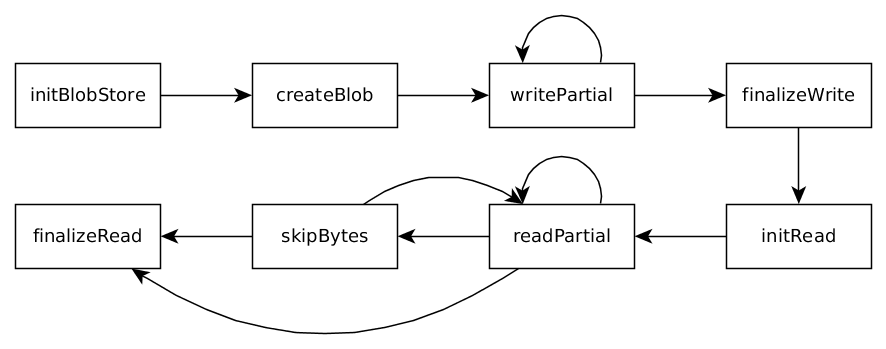
\includegraphics[scale=0.5]{figures/blob_operations_order.png}
\end{figure}

\section{Garbage Collection}
It is quite likely that the same blob would be shared by multiple ``values'' in the database. For a relational database these values are rows in a table, while for a document-oriented database, these values are documents.
Hence, we provide an interface for garbage collecting the deleted blobs.

\subsection{Starting the Garbage Collection}
The \texttt{startGC} method takes a BlobStore as argument and starts garbage collection (GC) for that BlobStore.
\texttt{startGC} does two things: It first renames the \textit{curr} folder to \textit{old} and then creates an empty \textit{curr} folder.
Once a GC has started you can not start another GC on the same BlobStore until the first one finishes - doing so will throw an error. Also, note that creation of new blobs and reading the old blobs can happen concurrently with the GC.

\begin{figure}[hbt]
  \caption{Directory structure of a BlobStore during GC}
  \label{fig:blobstore-dirstructure-gc}
  \dirtree{%
    .1 blobstore.
    .2 tmp.
    .3 1a4c5091-1295-4c9c-b8d3-8e6123a51b41.
    .2 old.
    .3 sha512-9b71d224bd62f3785d96d46ad3ea3....
    .2 curr.
    .3 sha512-11853df40f4b2b919d3815f64792e....
  }
\end{figure}

\subsection{Marking a blob as accessible}
Once a blob is marked as not deleted using the method \texttt{markBlobAsAccessible}, we move it from the \textit{old} folder to the \textit{curr} folder. This ensures that the blob does not get deleted at the end of the GC.

\subsection{End Garbage collection}
This step involves removal of all the blobs which are not accessible. The \texttt{endGC} method takes a BlobStore as argument and delete the \textit{old} subdirectory along with its contents.

\begin{table}[hbt]
\caption{Interface for garbage collection}
\label{tab:interface-gc}
\begin{center}
  \begin{tabularx}{0.91\textwidth}{lX}
    \hline\noalign{\smallskip}
    Methods & Purpose \\
    \noalign{\smallskip}
    \hline
    \noalign{\smallskip}
    \texttt{startGC} & Starts garbage collection for the given BlobStore\\
    \texttt{markBlobAsAccessible} & Marks the given blob as accessible\\
    \texttt{endGC} & Ends the garbage collection by removing all the unaccessible blobs\\
    \hline
  \end{tabularx}
\end{center}
\end{table}

\section{Concurrency}
In this section we will describe how the design described above allows concurrent access on blobs across processes.

\chapter{Conclusion}
\label{chap:conclusion}

\section{Summary}
In this thesis we described our design and implementation of Bloc - a library for handling large binary objects.
We also describe how our design achieves concurrency without using any locks.

\section{Future Work}
Currently our code uses several functions which are supported only on POSIX.
This means that our library will not work on Windows. In future, we might look
into adding support for Windows.

We are also working on creating a key-value store like Bitcask. We plan to add support for storing \texttt{BlobIds} provided by our library as a value in the key-value store.


\begin{singlespace}
\cleardoublepage
\addcontentsline{toc}{chapter}{References}
\renewcommand\bibname{References}
\printbibliography
\nocite{*}
\end{singlespace}

\end{document}
